\section{DeepCausality: A Framework for Hypergeometric Contextual Causal Reasoning}
\label{sec:deep_causality}

The pursuit of computational causality, aiming to imbue artificial intelligence with the ability to reason about cause and effect, stands at a critical juncture. While existing paradigms, surveyed in Section~\ref{sec:relaeted_work}, have provided invaluable foundational tools, they often operate within classical assumptions about spacetime and causal structure that are increasingly challenged by insights from modern physics and the complexities of real-world dynamic systems. The limitations of purely correlational AI, as discussed in Section~\ref{sec:motivation}, further underscore the need for frameworks that can move beyond statistical pattern matching towards a more fundamental representation of underlying generative mechanisms.

DeepCausality is engineered as a comprehensive, open-source computational causality framework in Rust, specifically designed to bridge this gap. It seeks to provide a robust system for constructing, executing, and managing explicit, context-aware causal models by drawing inspiration from a philosophical re-evaluation of causality itself, particularly the shift from a spacetime-dependent view towards an understanding of causality as an \textbf{effect propagation process} as detailed in Section~\ref{sec:causality_philosophy}. This re-evaluation, which considers the emergent nature of spacetime and the potential indefiniteness of causal order, motivates DeepCausality's core architectural choices.

The framework is built upon a design philosophy (Section~\ref{subsec:design_philosophy}) that prioritizes explicit mechanistic modeling, the deep primacy of context, and the operationalization of causal links. It aims to achieve a synthesis of causal understanding through three primary architectural pillars: a sophisticated \textit{Context Engine}, a versatile \textit{Causal Modeling Engine}, and integrated \textit{Causal State Machines}. By providing tools to model causality within rich, multi-dimensional, potentially non-Euclidean and dynamic environments, and by emphasizing the explicit articulation and verification of Observations and Assumptions, DeepCausality facilitates the development of more transparent, reliable, and adaptive intelligent systems capable of nuanced reasoning about cause and effect. This section details the core concepts, architecture, and implementation of this framework.

\subsection{Applied philosophical foundation}
\label{subsec:philosophical_motivations_architecture}

The architecture of DeepCausality is not merely a collection of data structures and algorithms; it is a direct response to the evolving understanding of causality, as explored in Section~\ref{sec:causality_philosophy}, and the practical limitations of existing computational approaches. The philosophical shift from a pre-defined spacetime stage for causal events towards causality as an emergent effect propagation process profoundly informs its design:

\begin{itemize}
    \item \textbf{Challenging Pre-existing Spacetime as a Fixed Background:} Traditional causality often assumes a fixed Euclidean spacetime where events unfold. Inspired by critiques from Leibniz to modern quantum gravity, which posit spacetime itself as relational or emergent, DeepCausality's \textbf{Context Engine} (Section~\ref{sec:deep_causality_context}) is designed with inherent flexibility. Its support for user-defined \textbf{Non-Euclidean Contexts} allows for the modeling of causal interactions within abstract relational spaces (e.g., networks, conceptual hierarchies) where "distance" and "connection" are not necessarily physical. This allows the "stage" for causality to be defined by the problem's intrinsic structure, rather than being confined to a default geometric interpretation.

    \item \textbf{Operational Causality and the Effect Propagation Process:} Russell's observation of physics focusing on evolving states rather than discrete cause-effect pairs \cite{Russell_Cause1912}, and Hardy's operational causaloids emerging from a more fundamental structure \cite{hardy2005probability}, inspire DeepCausality's core modeling primitives. The \textbf{Causaloid} (Section~\ref{subsubsec:causaloid}) embodies an operational, testable function representing a specific causal link or mechanism. The reasoning within a \textbf{CausaloidGraph} (Section~\ref{subsubsec:recursive_isomorphic_causal_structures}) then mirrors the concept of an \textit{effect propagation process}, where the activation of one Causaloid can influence others through defined (hyper)graph connections, representing the transfer of causal influence through the modeled system.

    \item \textbf{Emergent and Dynamic Causal Structures:} The notion from quantum gravity that causal order itself might be dynamic or emerge from underlying rules motivates the design for \textbf{dynamic context} (Section~\ref{sec:deep_causality_context}) and the envisioned capability for \textbf{dynamic CausaloidGraph adaptation} (discussed in Section~\ref{sec:advanced_modeling}). If the "generating function" for spacetime and causality is a deeper process, DeepCausality aims to provide tools to model systems where the causal rules themselves (the CausaloidGraph) can change in response to evolving context, reflecting how "effects emerge into being."

    \item \textbf{Explicit Assumption Management for Robustness:} Recognizing that all causal claims are conditional, the emphasis on first-class \texttt{Observation}, \texttt{Assumption}, and \texttt{Inference} types (Section~\ref{subsubsec:foundational_elements_formalism}) is a direct response to the need for rigor when moving from abstract causal theories to practical, verifiable models, especially when considering model transportability across diverse contexts (Section~\ref{subsubsec:foundational_elements_formalism}).
\end{itemize}

These philosophical underpinnings directly translate into an architecture that prioritizes explicit representation, contextual richness, and operational clarity, aiming to provide a more fundamental and adaptable toolkit for computational causality. The subsequent subsections detail the components of this architecture.


\subsection{Design Philosophy of DeepCausality}
\label{subsec:design_philosophy}

The architecture and implementation of DeepCausality are the result of a deliberate design philosophy refined through practical implementation, aiming to create a system that is expressive, performant, robust, and adaptable for complex causal reasoning tasks. Several core principles underpin the framework:

DeepCausality prioritizes the explicit encoding of known or hypothesized causal mechanisms within Causaloids. Crucially, it also provides first-class support for defining and managing observations from the empirical data and assumptions that encode the conditions under which causal claims are believed to hold true. This emphasis on explicit representation of mechanisms, the data that informs them, and the assumptions that bound them, is fundamental to achieving transparency, explainability, and a systematic approach to model validation and transfer. The operational nature of Causaloids, where each causal link is a testable function, ensures that the logic and its foundational assumptions are inspectable and verifiable through a defined Inference process.

A second core principle is the deep primacy of context. Recognizing that real-world causality is rarely context-free, DeepCausality elevates context from a set of conditioning variables to a rich, structured, and dynamic Context Hypergraph\footnote{\url{https://github.com/deepcausality-rs/deep_causality/blob/main/deep_causality/src/types/context_types/context_graph/mod.rs}}. This allows causal models to be deeply embedded within, and intricately responsive to, their operational environment, supporting multi-dimensional data (Data, Time, Space, SpaceTime), multiple distinct contexts, and both Euclidean and non-Euclidean relational information. This comprehensive contextualization aims for a faithful representation of reality.

The separation of causal logic from dynamic state emerged as a critical architectural decision. Distinguishing between the relatively stable causal mechanisms encoded in the CausaloidGraph\footnote{\url{https://github.com/deepcausality-rs/deep_causality/blob/main/deep_causality/src/types/reasoning_types/causaloid_graph/mod.rs}} and the evolving environmental state (managed by the Context Hypergraph) allows the CausaloidGraph to maintain efficient reasoning performance while reacting to real-time contextual changes. This design facilitates time-synchronous systems capable of operating on multi-scale temporal data.

Modularity and composability are also central. The recursive isomorphic nature of CausaloidGraphs enables hierarchical construction of complex models from simpler, reusable components, supporting an engineering approach to building large-scale causal systems. The trait-based design in the Rust implementation further enhances this, allowing for extension with custom data types and behaviors.

Finally, the choice of Rust as the implementation language reflects a commitment to performance, memory safety, and reliability—guarantees paramount for critical decision-making systems or high-throughput causal analytics. Rust's type system and trait mechanism are extensively leveraged to build an expressive yet efficient engine.

These guiding principles, including the foundational role of explicit observations and verifiable assumptions, collectively aim to provide a framework capable of representing complex causal knowledge in an understandable, maintainable, efficient, and robust manner, particularly for tackling the challenges of real-world dynamic systems and ensuring trustworthy causal inference.

\newpage

\subsection{Concepts of DeepCausality}
\label{sec:deep_causality_concepts}

DeepCausality's approach to computational causality is built upon several differentiating conceptual pillars, designed to offer enhanced expressiveness, flexibility, and operational capability compared to traditional methods. These core concepts underpin its architecture and enable its unique approach to modeling complex systems. At the forefront is a hypergeometric conceptualization of both context and causality, where relationships are not limited to pairwise interactions but can involve N-ary connections, represented via hypergraph structures. This allows for a more faithful modeling of group interactions and complex dependencies. Central to this is the Contextoid, an atomic unit capable of representing multidimensional contextual information, Data, Time, Space, and SpaceTime, including explicit support for both Euclidean and non-Euclidean geometries, and the Causaloid, an encapsulated, testable causal function forming the building block of causal models. These Contextoid are organized into recursive isomorphic CausaloidGraphs, permitting complex, layered causal models to be built modularly. The framework also emphasizes operational causality, where causal links are defined by executable functions, and direct intervention capabilities through Causal State Machines. Furthermore, the principle of multiple, adjustable contexts allows models to draw from and adapt to diverse, evolving information sources simultaneously, providing a level of contextual richness crucial for real-world applications. These concepts collectively enable DeepCausality to support the construction of deterministic, explainable, and deeply contextualized causal reasoning systems.

\subsubsection{Operational Causality}

While DeepCausality is compatible with insights from various causal inference schools, its core "Causaloid" structure is aligned with an operational view of causality, inspired by concepts such as Lucien Hardy's work on operational causality as foundation for quantum gravity \cite{hardy2005probability}. Instead of defining causality purely through statistical dependencies (e.g., conditional independence relations as in Bayesian Networks) or counterfactual contrasts alone, DeepCausality emphasizes the notion of a cause as an identifiable condition or process that, when active or present, leads to a specific effect or triggers a specific output through a defined function.

A causal link in DeepCausality is not merely an observed association but is encoded as a testable, executable function. This causal function takes input(observations, data from context) and evaluates whether a specific, predefined causal relationship holds true. If the conditions for the relationship are met, the function yields a positive result (e.g., true, or an "effect" being present); otherwise, it yields a negative result. This operational definition aligns with the scientific method in which hypotheses (causal links) are tested against evidence.

This perspective moves beyond simply asking "Are A and B related?" to asking "Does the presence of A, under context C, through a defined mechanism F, lead to B?". The mechanism F is explicitly encoded in the causal function. This is crucial because it makes the causal claim transparent, inspectable, and subject to refinement. While Hardy's work applies this to fundamental physics to understand the structure of spacetime events, DeepCausality adapts this operational spirit to model causal relationships in arbitrary complex systems. The "Causaloid" is the fundamental data structure that embodies this operational view of a single causal link.

\newpage

\subsubsection{Four Layers of Causal Reasoning}

DeepCausality's architecture conceptually maps to four interconnected layers of reasoning, providing a structured approach from raw data to causal understanding:

\begin{enumerate}
    \item \textbf{Observations}: This layer represents the raw data received from the environment – sensor readings, market prices, user inputs, etc. By themselves, observations are uninterpreted facts that lack intrinsic meaning. The corresponding observation\footnote{\url{https://github.com/deepcausality-rs/deep_causality/blob/main/deep_causality/src/types/reasoning_types/observation/mod.rs}} data type in Rust is the starting point for any reasoning process.
    
    \item \textbf{Assumptions}: Causal reasoning, unlike some purely data-driven methods, relies on explicit and, importantly, testable assumptions. These assumptions provide the frame of reference for interpreting observations. They might concern the reliability of data sources, the expected range of values, or preconditions that must hold for a causal model to be applicable. Deep causality provides a designated Assumption\footnote{\url{https://github.com/deepcausality-rs/deep_causality/blob/main/deep_causality/src/types/reasoning_types/assumption/mod.rs}} type to encode and test explicitly stated assumptions. 
   
    \item \textbf{Inferences}: This layer involves deriving insights or conclusions from observations under the stated assumptions. It's about interpreting the raw data in light of what is assumed to be true. This is where patterns are identified and initial judgments are made. DeepCausality's documentation highlights that even at this stage, one can estimate the ratio of inferable, inverse-inferable (absence of cause associated with absence of effect), and non-inferable observations, which provides early clues about the strength of potential causal links. DeepCausality encapsulates inference in a dedicated Inference\footnote{\url{https://github.com/deepcausality-rs/deep_causality/blob/main/deep_causality/src/types/reasoning_types/inference/mod.rs}} type to streamline inferences from observations.

    \item Causality: This is the layer in which established causal relations govern subsequent inferences. A causal relation, often expressed as (\textit{IF} $A$ \textit{THEN} $E$, \textit{AND IF NOT} $A$ \textit{THEN NOT} $E$), is typically established after rigorous testing at the inference layer (e.g., observing a high co-occurrence of $A$ with $E$, and NOT $A$ with NOT $E$). Once a causal relationship is considered to hold (e.g., IF pressure $>$ threshold THEN valve\_failure\_imminent), it becomes a rule that dictates the results for future matching observations.
\end{enumerate}

DeepCausality's core types (Observation, Assumption, Inference, Causaloid) and their associated reasoning traits directly map to these conceptual layers, providing a structured way to build causal models.

\subsubsection{Hypergeometric Representation}

The term "hypergeometric" in DeepCausality refers to its reliance on graph-theoretic structures, specifically hypergraphs, to represent both context and causal relationships. This is a deliberate design choice that offers several advantages over purely algebraic or flat relational models.

\textbf{Simplifying Complexity:} Modeling complex causality can lead to either complex algebra with simple structures or simple arithmetic with complex structures. DeepCausality opts for the latter, believing that structural complexity is more manageable and scalable through computational graph techniques than highly intricate algebraic formulations, especially when dealing with hundreds or thousands of interacting causal factors.

\textbf{Explicit Relationships:} Hypergraphs allow for the explicit representation of N-ary relationships, where an edge (hyperedge) can connect any number of nodes. This is more expressive than simple graphs for modeling complex dependencies, such as multiple conditions leading to a single effect, or a single cause influencing multiple effects through different pathways.

\textbf{Recursive Composability:} A key feature is that nodes within these hypergraphs can themselves be entire sub-graphs. A CausaloidGraph can have nodes that are individual Causaloids or other CausaloidGraphs. This recursive isomorphism allows for hierarchical and modular construction of highly complex causal models, breaking them down into manageable, understandable, and reusable components.

\textbf{Identifiable Reasoning Paths:} Reasoning over a graph structure allows for the tracing of "explanation paths" – the sequence of activated causaloids and contextual data points that led to a particular conclusion. This is fundamental to DeepCausality's end-to-end explainability.

By representing both context and causal models as hypergraphs, DeepCausality creates a unified structural approach for describing and reasoning about complex, interacting systems.

\newpage

\subsection{Context}
\label{sec:deep_causality_context}

The context is a foundational element that enables causal models to be grounded in the specifics of a given situation and to handle diverse, dynamic, and multi-faceted contextual information. It allows DeepCausality to move beyond simplistic causal models towards systems that can understand and react to the nuanced, multi-dimensional, and dynamic nature of the environments in which they operate. It is the foundation upon which deeply contextualized and therefore more accurate and relevant causal inferences can be built. The core elements that comprise context in DeepCausality:

\textbf{Contextoids}: 

The primary building block for context is the Contextoid. Each Contextoid is a node in a context hypergraph and encapsulates a single unit of contextual information. DeepCausality defines four primary types of contextoids:

\begin{enumerate}
    \item \textbf{Data Contextoid}: Stores arbitrary data of a generic type T. This can be a raw sensor reading, a calculated metric, a textual feature, or any other piece of information relevant to the causal model.
    \item \textbf{Time Contextoid}: Represents a unit of time, specified by a TimeScale (e.g., Year, Month, Day, Nanosecond) and a time value of type T (typically an unsigned integer).
    \item \textbf{Space Contextoid}: Represents a unit of space, potentially with up to three coordinates (X, Y, Z) of type T. This does not inherently carry unit information (e.g., meters vs. feet), which must be managed by the application logic.
    \item \textbf{SpaceTime Contextoid:} Combines spatial and temporal information, representing a unit of space at a specific unit of time. For example, in a drone application, a SpaceTime contextoid could represent the drone's GPS coordinates (lat, lon, alt) at timestamp in nanosecond resolution. Multiple sensor readings (Data contextoids) could then be linked to this single SpaceTime contextoid, indicating they were all taken at the same place and time
\end{enumerate}

\textbf{The Context Hypergraph}: 

Individual contextoids are organized into a Context object, which is internally represented as a hypergraph. Nodes are contextoids, and hyperedges represent relationships between them. This structure allows for flexible and complex contextual models because real-world causality rarely occurs in a vacuum; it is almost always conditioned by, and interacts with, a complex web of surrounding circumstances, historical states, and environmental factors. The Context Hypergraph provides the means to explicitly model this intricate web, making it an active and integral part of the causal reasoning process itself.

The choice of a hypergraph over a simple graph or other data structures is deliberate and offers significant advantages for representing complex contextual relationships:

\begin{enumerate}
    \item \textbf{Representing N-ary Relationships:} Unlike simple graphs where an edge connects only two nodes, a hyperedge in a hypergraph can connect an arbitrary number of nodes. This is crucial for context because many contextual situations involve relationships between more than two entities.
    \item \textbf{Flexibility and Expressiveness:} Hypergraphs are highly flexible and can represent a wide variety of relational structures, including simple graphs, hierarchical structures, and overlapping sets, all within a unified framework. This allows the Context Hypergraph to adapt to the diverse ways contextual information is structured in different domains.
    \item \textbf{Modularity and Composition:} Portions of a context hypergraph can represent distinct but related contextual facets (e.g., a sub-hypergraph for weather conditions, another for economic indicators). These can be reasoned over separately or their interrelations can be explicitly modeled with hyperedges connecting nodes across these sub-graphs.
\end{enumerate}

\newpage

\subsubsection{Adjustable Protocol:}

A core challenge in modeling real-world systems with causal inference is the inherent dynamism of their operational environments; contextual factors are rarely static, as sensor readings drift, market conditions fluctuate, and environmental parameters change. To ensure that causal models remain relevant and accurate over time, the contextual information they rely upon must possess a degree of plasticity. DeepCausality addresses this necessity through its Adjustable protocol, as detailed in its conceptual\footnote{https://deepcausality.com/docs/concepts/} and architectural\footnote{https://deepcausality.com/docs/architecture/} documentation. This protocol is a mechanism designed to provide a uniform and controlled way of modifying the internal state of Contextoids within the Context Hypergraph, even within structurally static contexts.

The Adjustable protocol is conceptualized as an optional extension to the fundamental Contextoid types, namely Data, Time, Space, and SpaceTime. By default, Contextoids are immutable post-instantiation, a design choice that promotes data integrity and predictability, particularly in certain audited or foundational contextual layers  "Non-adjustable means that, after instantiation, the structure is immutable..."\footnote{https://deepcausality.com/docs/concepts/}. However, when contextual elements must reflect ongoing changes, their corresponding Contextoid types can implement the Adjustable trait. This trait defines a specific interface for sanctioned mutations, thereby allowing the values encapsulated by a Contextoid to be altered without changing the Contextoid's identity—its unique ID within the hypergraph—or its established relational linkages, which are the hyperedges.

The Adjustable protocol primarily exposes two optional methods that implementing types can choose to override. The first method, $update(new_value)$, is conceptualized as the mechanism for replacing the existing value within a Contextoid with entirely new data. This is typically invoked when fresh information becomes available from an external source or as the result of an internal calculation. For instance, a Data Contextoid representing the "latest stock price" would have its update() method called each time a new price tick is received from a market data feed. Similarly, a SpaceTime Contextoid tracking a moving object would be updated with new coordinates and a new timestamp as the object's position changes. The crucial aspect is that the update() method signifies a complete replacement, reflecting the most current state of that particular contextual element.

In contrast, the second method, $adjust(adjustment_factor)$, is designed for corrections, relative modifications, or incremental changes to the existing value within a Contextoid. This is particularly useful when the current value needs to be refined based on new information, a known bias, or an influencing factor, rather than being wholly superseded. For example, a sensor reading encapsulated in a Data Contextoid might be subject to a known calibration drift over time; an adjust() method could therefore apply a correction factor to mitigate this drift. In more complex scenarios, such as the spatio-temporal adjustments required for gravitational effects mentioned in the documentation\footnote{https://deepcausality.com/docs/concepts/}, the adjust() method might take a more complex $adjustment_factor$, for instance, an ArrayGrid\footnote{https://deepcausality.com/blog/the-grid-type/} representing a transformation matrix, to modify the internal coordinates or temporal values of AdjustableSpaceTime Contextoids.

The protocol's design intentionally makes these methods optional by providing empty default implementations. This allows implementers to provide only the functionality that is strictly required by their specific Contextoid type. If a Contextoid only ever needs to be fully updated with new values, only the update() method needs to be implemented, thus promoting minimalism and avoiding unnecessary code.

The significance of the Adjustable protocol for handling evolving environments is multi-fold. Firstly, it provides a uniform interface for mutation across different types of Contextoids—be they standard (Data, Time, Space, SpaceTime) or custom user-defined contextoid types—so long as they implement the protocol. This uniformity simplifies the design of higher-level context management systems that need to interact with a heterogeneous collection of contextual elements. Secondly, it facilitates a decoupling of the update logic from the core context structure. DeepCausality deliberately does not provide a global context update mechanism by default. Instead, it provides the means for updates via the Adjustable protocol and wisely leaves the strategy of when and how to apply these updates to the application developer. This is a critical design decision, recognizing that the correct order and timing of updates can be highly domain-specific and are crucial for maintaining consistency, especially when dealing with multiple interacting data streams or inter-dependent contextual variables.

Thirdly, the Adjustable protocol is essential for facilitating real-time responsiveness. By allowing Contextoids to be updated or adjusted efficiently, causal models that query the Context Hypergraph can access the most current state of the environment. This is fundamental for real-time decision-making systems that must react promptly to emergent changes. 

Finally, the protocol-based approach is inherently future-proof and extensible. If new types of mutations or contextual operations become necessary, such as a hypothetical delete() operation for contextual data, the Adjustable protocol could be extended with new method signatures and empty default implementations. Custom Contextoid types implementing these new methods would then remain compatible with the overall context management framework, ensuring long-term adaptability of the system.

The Adjustable protocol endows DeepCausality's Context Hypergraph with the necessary plasticity to accurately mirror evolving realities. It allows contextual information to be a living representation of the environment, continuously refined and updated, thereby ensuring that the causal reasoning performed upon it remains grounded, relevant, and capable of driving adaptive behavior in dynamic systems. This capacity for controlled mutability within the contextual layer is a key enabler for building causal models that are not just static representations of knowledge but active participants in understanding and responding to a continuously changing world.

\subsubsection{Multiple Contexts}

A significant advancement in DeepCausality, introduced from version 0.6 onwards is its architectural capacity to allow causal models to utilize multiple distinct contexts simultaneously. This capability transcends the already powerful notion of a single, rich Context Hypergraph by enabling a system to maintain and draw upon several independent or interrelated contextual realms. This feature is a significant enhancement to the framework's representational power, crucial for modeling systems where causality is influenced by diverse, potentially disjoint, yet concurrently relevant sets of information.

Prior to this enhancement, while a single Context hypergraph could be internally complex and multi-faceted, all contextual information accessible to a given causal model had to reside within that unitary structure. The introduction of multiple contexts allows a causal model, specifically the causal function within a Causaloid, to be endowed with the ability to reference and query data from several different contexts, each with its own unique ID, structure, and set of Contextoids. This fundamentally alters the landscape for modeling intricate real-world scenarios where different types of contextual information might be best organized, updated, or conceptualized separately, yet all contribute to a holistic causal understanding.

The practical implementation\footnote{https://deepcausality.com/blog/announcement-multiple-contexts/} of this feature involves an Application Programming Interface (API) where additional contexts can be created and assigned unique identifiers. A causal model can then be designed to specifically target these different context IDs when it needs to fetch particular pieces of contextual data. This means a single \texttt{causal\_function} might, for instance, retrieve temporal information from \texttt{Context\_ID\_1} (perhaps a master timeline), spatial data from \texttt{Context\_ID\_2} (a geographical information system context), and specific sensor readings from \texttt{Context\_ID\_3} (a real-time data stream context), all within the course of evaluating a single causal hypothesis.

The importance of managing multiple distinct contexts is best understood through concrete application domains where such separation and selective integration are natural and powerful. The documentation\footnote{https://deepcausality.com/blog/announcement-multiple-contexts/} allude to several such scenarios. Consider the financial industry, particularly in the modeling of synthetic instruments like future spreads. A spread's behavior is intrinsically tied to the behavior of its constituent legs (e.g., a long-term future contract and a short-term future contract) as well as the characteristics of the spread itself. With multiple contexts, a DeepCausality system can maintain \texttt{Context\_LongLeg} containing all relevant data for the long-term contract (its price series, volatility, specific news events impacting it), a \texttt{Context\_ShortLeg} for the short-term contract, and a \texttt{Context\_Spread} containing derived data like the price differential, historical spread volatility, and perhaps arbitrage opportunity indicators. A causal model designed to predict spread behavior or identify trading opportunities can then intelligently query all three contexts, drawing precisely the information needed from each distinct source to make a robust inference. Attempting to meld these fundamentally different, though related, information sets into a single, monolithic context graph could lead to an overly complex and less maintainable structure.

Similarly, in the Internet of Things (IoT) domain, an advanced industrial monitoring system might involve sensor networks deployed across different physical plants or monitoring entirely different types of processes. One Context could represent the environmental sensor data (temperature, humidity) from Plant A, while another Context represents the operational parameters (machine RPM, energy consumption) from specialized machinery in Plant B, and yet another Context might track overall supply chain logistics data relevant to both. A higher-level causal model assessing overall production risk or efficiency could then tap into these distinct contextual sources. Each context can be updated independently based on its own data streams and lifecycle, yet their information can be synergistically combined at the point of causal reasoning.

This multi-context architecture also enhances modularity and scalability. Different teams or modules within a larger system could be responsible for maintaining and updating specific contexts relevant to their domain of expertise. For example, a meteorological team might maintain a detailed \texttt{WeatherContext}, while an economic analysis team maintains an \texttt{EconomicIndicatorContext}. A causal model predicting agricultural output could then be configured to utilize both, without either team needing to understand the full intricacies of the other's contextual data, as long as clear interfaces for querying relevant \texttt{Contextoids} are defined.

The crucial design element enabling this is that the causal function within a Causaloid receives an immutable reference not just to \textit{a} context, but to an overarching context management system that can resolve queries to \textit{specific, identified} contexts. The API allows for setting a "current" additional context for operations, and for checking the existence and retrieving data from any named or ID-referenced context\footnote{https://deepcausality.com/blog/announcement-multiple-contexts/}. This ensures that while the causal logic can be complex and draw from diverse sources, the process remains explicit and manageable.

The support for multiple distinct contexts elevates DeepCausality from a framework for reasoning within a single rich world-model to one capable of reasoning across a federation of specialized world-models. This mirrors how complex human reasoning often draws upon distinct but relevant bodies of knowledge. It is a sophisticated feature that significantly extends the framework's capacity to model the intricate, multi-faceted causal tapestries found in complex systems, providing a more organized, maintainable, and expressive foundation for advanced causal inference.

\subsubsection{Euclidean and Non-Euclidean Contexts:}


A particular aspect of DeepCausality's architecture is its sophisticated handling of the geometric nature of contextual information, explicitly accommodating both Euclidean and Non-Euclidean Contexts. This dual capability significantly broadens the framework's applicability. It allows DeepCausality to model causality in domains where relationships are defined by abstract connectivity or  conceptual similarity rather than solely by physical proximity in a metric space.

Traditionally, spatial context in computational models often defaults to a Euclidean interpretation, wherein entities are located by coordinates in a one, two, or three-dimensional space, and relationships such as distance are defined by standard metrics. DeepCausality provides robust support for such conventional representations. Its default \texttt{Space} Contextoid, for instance, can store up to three coordinates (X, Y, Z) of a generic type \texttt{T}, and the \texttt{SpaceTime} Contextoid naturally extends this to incorporate a temporal dimension. This approach is perfectly suitable for a vast range of applications, such as modeling the physical layout of a sensor network, the trajectory of an autonomous drone, or the geographical distribution of environmental factors. In these scenarios, causal influences might indeed propagate based on physical distance or containment within defined spatial regions.

However, the profound innovation within DeepCausality lies in its explicit recognition that many crucial contextual relationships are not inherently Euclidean. Consider social networks, where influence propagates along ties of friendship or collaboration, not necessarily physical nearness. Think of biological systems, where proteins interact based on specific binding sites and pathway memberships, forming a complex interaction network. Forcing such inherently non-Euclidean relationships into an ill-fitting Euclidean vector space can lead to a significant loss of fidelity, the introduction of artificial constraints, or an obscuring of the true underlying causal pathways, a concern echoed by J.M. Bishop \cite{bishop2020artificialintelligencestupidcausal} regarding the limitations of Euclidean representations in Artificial Intelligence.

DeepCausality's architecture addresses this challenge through its flexible, trait-based design, particularly the \texttt{Spatial<V>} trait. This trait defines a protocol---a set of methods that a type must implement to be considered "spatial" within the framework---but it crucially \textit{does not mandate a Euclidean interpretation} for how those methods are implemented or what constitutes a "spatial" relationship. While the default \texttt{Space} structure provides a convenient Euclidean implementation, users are empowered to create custom types that implement the \texttt{Spatial<V>} protocol to embody entirely non-Euclidean or abstract notions of "space" and "relationship."

For instance, a custom type named \texttt{SocialGraphNodeContext} could implement \texttt{Spatial<UserID>}, where methods like \texttt{get\_neighbors()} would return directly connected users in a social network graph, and a "distance" metric, if defined, might represent degrees of separation. Similarly, a \texttt{CorrelationClusterContext} could implement \texttt{Spatial<AssetID>}, where its methods define adjacency or proximity based on assets exceeding a certain correlation threshold or belonging to the same statistically derived cluster. Another example might involve a \texttt{SectorGraphContext} implementing \texttt{Spatial<NodeId>} for an industry classification graph, where relationships are defined by graph connectivity. The core DeepCausality reasoning engine, when interacting with context via the CausaloidGraph, remains agnostic to the specific underlying geometry. It requests spatial information or evaluates relationships through the standardized \texttt{Spatial<V>} trait methods; the concrete implementation provided by the custom Contextoid type---whether it is based on Cartesian coordinates, graph adjacencies or conceptual hierarchy links---determines the nature of the "space" through which causal effects are considered to propagate.

\newpage

The significance of this design lies in its ability to model causality directly within the most relevant relational structure of the domain under study. It obviates the need to artificially project complex, abstract dependencies onto a potentially unsuitable geometric substrate. Instead, the domain's natural topology, be it a network, a feature space manifold, a categorical hierarchy, or a conceptual map, can be directly represented and reasoned over. This allows the causal functions within Contextoid to operate on concepts like "influence," "similarity," "membership," or "connectivity" as primary contextual factors, leading to more faithful, insightful, and potent causal models.

Furthermore, the uniformity provided by the trait system means that these diverse spatial and relational conceptualizations can coexist and interact within a single, comprehensive DeepCausality application. A causal model might simultaneously draw upon a Euclidean \texttt{SpaceTime} context representing the physical location of an event and a non-Euclidean \texttt{SocialInfluenceContext} representing the network of actors involved. This capacity to fluidly integrate and reason across different conceptualizations of space and relationship, all grounded within a rigorous causal framework, unlocks a profound potential for understanding and modeling systems based on new and unique contextual capabilities.

\subsubsection{Contextual capabilities:}

In DeepCausality, context intrinsically becomes an active and integral part of the causal reasoning process itself and enables variety of capabilities. 

\textbf{Enables Deep Contextualization: }
The primary importance is that it allows causal models (Causaloids) to be deeply and specifically contextualized. Instead of a causal rule operating on global variables or a simple set of parameters, it can query a rich, structured context for precisely the information it needs, relevant to the current observation's time, location, or other defining characteristics.
For example, a causal rule for assessing crop yield might perform very differently in "Drought" conditions versus "AdequateRainfall" conditions. The Context Hypergraph can explicitly represent these conditions (perhaps as Data or Symbolic Contextoids), and the Causaloid can query the current weather context before making its inference.

\textbf{Grounds Abstract Causal Rules in Concrete Reality:} Abstract causal relationships ("IF A THEN B") gain practical meaning and applicability only when A and B can be mapped to specific, observable, and contextually relevant phenomena. The Context Hypergraph serves as this mapping layer, providing the concrete instantiations of variables and conditions that the causal rules operate upon.

\textbf{Supports Reasoning Across Multiple Dimensions and Resolutions:} Because Contextoids can represent Data, Time, Space, and SpaceTime, the Context Hypergraph allows causal models to reason about phenomena that unfold across these dimensions. For example, a model for urban traffic flow might consider current traffic density (Data), time of day (Time), specific road segments (Space), and sensor readings from particular intersections at particular times (SpaceTime).

\textbf{Facilitates Dynamic and Adaptive Reasoning:} With Adjustable Contextoids, the Context Hypergraph is not static; it can evolve in real-time as new information arrives or as the environment changes. Causal models querying this dynamic graph will therefore adapt their reasoning to the most current state of the world.

\textbf{Manages Complexity in Multi-Factor Systems: }Many real-world systems are influenced by a multitude of interacting factors. The Context Hypergraph provides a way to organize this complexity, making it explicit and accessible to the causal model. This prevents causal rules from becoming overly complex by having to manage all contextual variations internally; instead, they can delegate contextual queries to the specialized context.

\textbf{Enables Non-Euclidean Relational Context: }As stressed previously, the ability of the context (and its underlying Spatial<V> trait) to represent non-Euclidean relationships is a profound advantage. This means the "space" in which causes operate can be a social network, a conceptual hierarchy, a correlation matrix, etc. The Context Hypergraph provides the structure to define these abstract "contextual landscapes."

\newpage

\subsection{Causality}
\label{sec:deep_causality_causality}

While the Context Engine provides the rich, structured environmental grounding, the core causal reasoning within DeepCausality is performed by its versatile Causal Modeling Engine. This engine is designed to move beyond purely statistical or algebraic formulations of causality, opting instead for a structural and operational conceptualization. It facilitates the construction of explicit causal models through composable units of causal logic that operate within the rich environments provided by the Context Engine. Key to this engine are the concepts of the Causaloid, the mechanism of contextual causal reasoning, and the powerful paradigm of recursive isomorphic causal data structures embodied in the CausaloidGraph.

\subsubsection{The Causaloid: A Unit of Causation}
\label{subsubsec:causaloid}

The fundamental building block for expressing causal relationships within DeepCausality is the Causaloid, a concept inspired by Lucien Hardy's work in operational physics aimed at formalizing cause-and-effect in physical systems \cite{hardy2005probability, DeepCausalityWebsite}. In DeepCausality, a Causaloid is adapted to serve as an encapsulated, operational unit that encodes a single, testable causal hypothesis or a specific causal mechanism. As described in section \ref{sec:deep_causality_concepts}, each Causaloid is defined by a \textbf{causal function} ($f_\chi$ in our formalism, Section \ref{subsec:formal_specification}). This function takes an input observation (e.g., data representing a potential cause or a system state) and, critically, can receive an immutable reference to one or more Context hypergraphs. The causal function then executes specific logic to determine whether, given the observation and the relevant contextual information, the posited causal relationship holds or the cause is considered active. Typically, this evaluation results in a Boolean outcome (true/active or false/inactive), thereby providing a deterministic assessment of the individual causal link.

This operational definition is pivotal. Instead of representing a cause as a mere statistical dependency or an abstract node in a graph whose meaning is externally imposed, the Causaloid internalizes the logic of the causal link itself. This makes the causal assertion explicit, inspectable, and directly testable. For instance, a Causaloid designed to detect a 'golden cross' in financial markets would encapsulate a function that accesses specific moving average values (from \texttt{Data Contextoids}) linked to relevant time points (from \texttt{Time Contextoids}) within a financial market Context, and then applies the mathematical criteria for a golden cross. This explicit encoding of the mechanism within the Causaloid's function is a core tenet that supports the framework's emphasis on explainability.

\subsubsection{Contextual Causal Reasoning}
\label{subsubsec:contextual_causal_reasoning}

A defining feature of DeepCausality, setting it apart from many traditional causal modeling approaches, is its deep and intrinsic integration of context into the reasoning process \cite{DeepCausalityWebsite}. Contemporary computational causality often assumes that the modeled causal relations constitute the entirety of the model, or treats context as simple conditioning variables. DeepCausality, however, elevates context from a passive backdrop to an active, structured entity---the Context Hypergraph as detailed in Section~\ref{sec:deep_causality_context}---that actively participates in the evaluation of causal relationships.

As outlined in section \ref{sec:deep_causality_concepts} is achieved by providing the causal function within each Causaloid with an immutable reference to the relevant Context instance(s) (see $C_{refs}$ in the formalism, Section \ref{subsec:formal_specification}). This allows the causal logic to be highly adaptive and specific to the circumstances. The causal function can dynamically query the Context Hypergraph for any Contextoid (Data, Time, Space, SpaceTime) or relational information it requires to make its determination. For example, a causal model for a physical system might have Causaloids whose functions query SpaceTime Contextoids for location and time, Data Contextoids for ambient temperature or pressure from the same spatio-temporal vicinity, and then evaluate a physical law based on these contextualized inputs.

The framework's support for multiple contexts, as discussed in Section~\ref{sec:deep_causality_context}, further enriches this capability. A single Causaloid can be designed to draw information from several distinct Context Hypergraphs, each representing different facets of the environment or different sources of information (e.g., one context for market data, another for news sentiment, a third for macroeconomic indicators). This allows for the construction of models that reason holistically across diverse, yet relevant, information domains. Diagram \ref{fig:contextual_causal_model} labeled "Contextual Causal Model" illustrates how specific Causaloids within a larger model can be contextualized by accessing data from a shared Context, while others might remain context-free if their logic is purely observational or self-contained. This selective contextualization provides fine-grained control over how environmental factors influence specific causal links within a broader model.

\newpage

\subsubsection{Recursive Isomorphic Causal Data Structures: The CausaloidGraph}
\label{subsubsec:recursive_isomorphic_causal_structures}

To scale from simple causal links to arbitrarily complex causal systems, DeepCausality employs a powerful structural paradigm: recursive isomorphic causal data structures, primarily realized through the CausaloidGraph\footnote{https://deepcausality.com/docs/concepts}. While individual Causaloids represent atomic causal hypotheses, the CausaloidGraph allows these units to be organized into intricate networks that model complex causal interdependencies (formalized in Section~\ref{subsubsec:causaloid_graph_formalism}).

A CausaloidGraph is itself a hypergraph where each node represents a causal element. The "recursive isomorphic" nature, a key innovation visually depicted in Figure~\ref{fig:causaloid_diagram}, means that a node ($v_g$) within a CausaloidGraph ($G$) is not restricted to being only a simple, elementary Causaloid. Instead, the payload of such a node ($\text{payload}_g$) can encapsulate:
\begin{enumerate}
    \item A single, elementary \texttt{Causaloid} ($\chi$).
    \item A collection of Causaloids (e.g., implemented as a `CausalArray`, `CausalHashMap`, `CausalVector`, or `CausalVecDeque` where the collection itself might have an aggregate evaluation logic (e.g., "activate if any causaloid in this collection is active").
    \item Another entire CausaloidGraph ($G'$), effectively creating a sub-model or a nested causal structure.
\end{enumerate}

\begin{figure}[H] % Or [htbp] for more flexibility
    \centering
    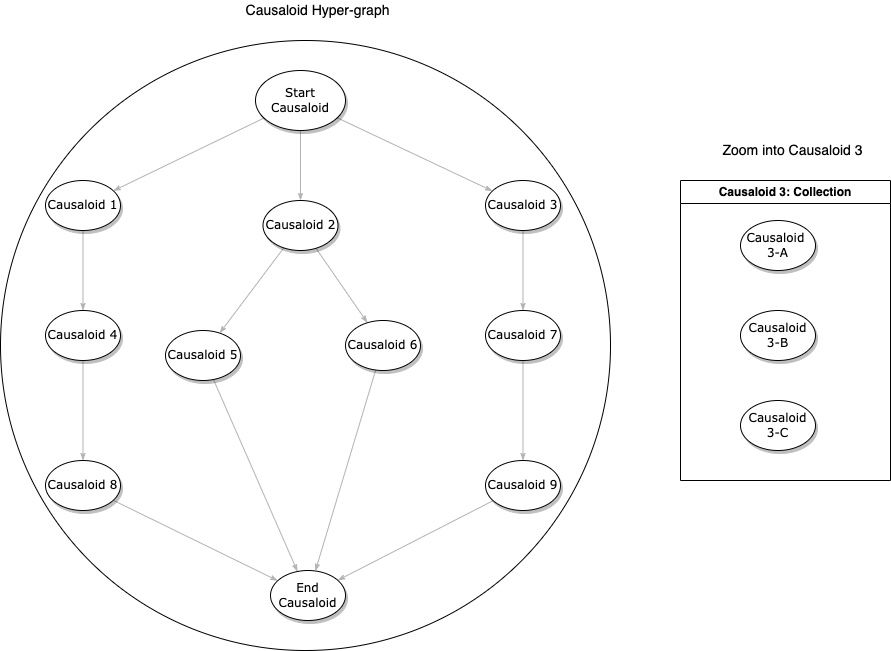
\includegraphics[width=0.8\textwidth]{img/causaloid.png} % Adjust width as needed
    \caption{The Causaloid Diagram illustrating the recursive isomorphic structure of a CausaloidGraph. Nodes within the graph can be elementary Causaloids, collections of Causaloids, or even encapsulate entire sub-\texttt{CausaloidGraphs}, enabling hierarchical and modular causal model construction. }
    \label{fig:causaloid_diagram}
\end{figure}

This recursive definition, as illustrated in Figure~\ref{fig:causaloid_diagram}, allows for a highly modular and hierarchical approach to building complex causal models. Macro-level causal phenomena can be represented by high-level nodes in a graph, and these nodes can then be decomposed into more detailed sub-graphs representing the interacting micro-level causal mechanisms that constitute the higher-level effect. This "transparent composability" \footnote{https://deepcausality.com/docs/concepts} means that a complex system can be broken down into understandable, manageable, and potentially reusable causal modules.

\newpage

Reasoning over a CausaloidGraph involves evaluating its constituent causal elements and propagating their activation states according to the (hyper)edges ($E_G$) that define their logical interdependencies ($\text{logic}_e$). DeepCausality supports various reasoning modes over the graph, such as reasoning over the entire graph, a specific Causaloid node, a defined sub-graph between start and stop nodes, or along the shortest path between two Causaloids. The activation state of a Causaloid (once active, it typically remains so until negatively re-evaluated based on new inputs) allows the graph to maintain a memory of which causal conditions have been met, facilitating reasoning over evolving states based on changing input data and context.

Contextualized causal reasoning is implemented by passing an immutable reference implicitly into the causal function. This mechanism also allows us to contextualize certain Causaloids while leaving others context-free if this is a desirable option. The diagram below, Figure~\ref{fig:contextual_causal_model}, shows this scenario in which specific Causaloids use data from a Context while other Causaloids remain context-free.

\begin{figure}[H] % Or [htbp] for more standard float behavior
    \centering
    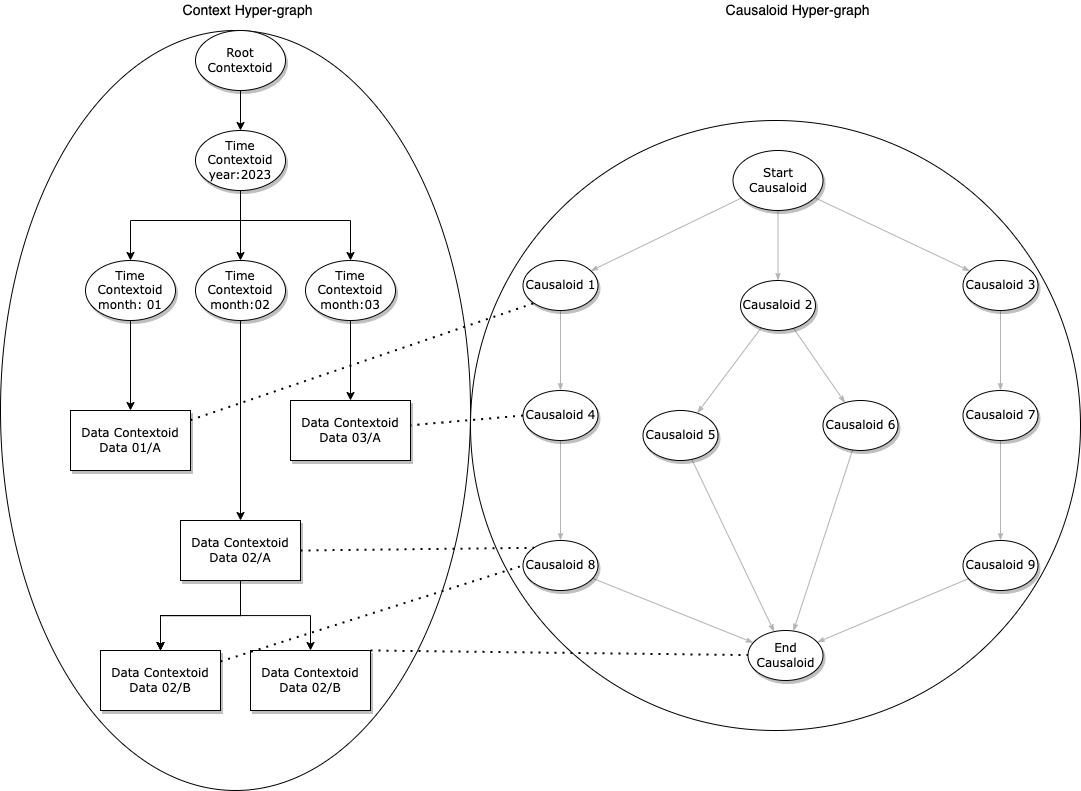
\includegraphics[width=0.9\textwidth]{img/contextual-model.png} % Adjust width as needed
    \caption{Illustration of a Contextual Causal Model in DeepCausality. Specific \texttt{Causaloids} are shown interacting with an external \texttt{Context}  drawing contextual data to inform their evaluation. Other \texttt{Causaloids} operate without direct contextual input, demonstrating the flexibility of selective contextualization.}
    \label{fig:contextual_causal_model}
\end{figure}

This structural approach, combining operational Causaloids with deeply contextualized reasoning and recursively composable CausaloidGraphs, provides DeepCausality with a robust and expressive engine for modeling and executing complex causal knowledge.

\newpage

\subsection{Causal State Machine}
\label{subsec:csm}

A crucial further step for many practical causality based applications is the translation of these causal insights into tangible actions or interventions. The \textbf{Causal State Machine (CSM)} is the component within DeepCausality specifically engineered to bridge this gap, enabling a direct and deterministic linkage from identified causal conditions to predefined operational responses. This facilitates the creation of dynamic control, supervision, and autonomous decision-making systems grounded in explicit causal logic.

The conventional view of causal models often separates the modeling process from subsequent intervention, primarily for reasons of flexibility and analytical clarity. While this separation remains valid and useful for many analytical or exploratory use cases, it can be suboptimal for systems requiring tight, deterministic coupling between causal understanding and immediate action, such as in dynamic control systems or automated supervision. Traditional finite state machines (FSMs), often employed in control systems, typically require all possible system states to be known upfront. However, with the advent of cloud-native applications and other dynamically evolving systems, such as those involving programmatically managed software services or parametric causal models that are brought online and offline dynamically, the complete set of system states may not be known at design time. This limitation restricts the applicability of conventional FSMs.

DeepCausality's CSM offers a more flexible and powerful paradigm. It generalizes the concept of a state machine by defining states not merely as arbitrary system configurations, but specifically as \textit{identified causes} or \textit{combinations of causes} becoming active within one or more supervised CausaloidGraphs. When a particular causal state is recognized through the evaluation of the associated causal model(s) against current observations and context, the CSM is designed to trigger a specific, predefined action or intervention that leads to a desired effect or system adjustment\footnote{https://deepcausality.com/docs/csm}. The core architecture of a CSM in DeepCausality involves this explicit mapping:
\begin{itemize}
    \item \textbf{Causal States}: A state within the CSM corresponds to a specific pattern of activation across one or more Causaloids in the supervised CausaloidGraph(s). This could be a single Causaloid becoming active (e.g., ``Sensor\_Pressure\_Exceeds\_Threshold'') or a more complex logical combination of multiple Causaloid activations (e.g., ``(Smoke\_Detected AND Temperature\_Rising) OR Emergency\_Override\_Signal\_Active'').
    \item \textbf{Deterministic Actions}: Each defined causal state is linked to a deterministic action. These actions are typically implemented as regular Rust functions, which allows for arbitrary complexity. An action could range from simple logging or alerting, to modifying the system's operational parameters, adjusting context variables for downstream models, triggering external API calls, or initiating complex control sequences.
\end{itemize}
A key characteristic of the CSM is its potential for dynamic configuration\footnote{https://deepcausality.com/docs/intro}. Unlike traditional FSMs, a DeepCausality CSM does not necessarily require all possible causal states and their corresponding actions to be enumerated at the initial design phase. Instead, as new components, systems, or causal hypotheses (represented by new Causaloids or CausaloidGraphs) are introduced or come online, their relevant causal states and associated actions can be dynamically registered with the supervising CSM. For instance, if a system being monitored (e.g., an industrial plant) has new sensors added, the causal rules pertaining to these sensors and the actions to be taken upon their triggering specific conditions can be seamlessly integrated into the existing CSM structure. This allows the CSM to adapt and extend its supervisory capabilities as the system it monitors evolves. 

The CSM, therefore, acts as an orchestrator, as formalized in Section \ref{subsubsec:csm_formalism}. It can manage the flow of information by triggering data extraction from relevant Contextoids, ensuring these updates inform the supervised causal models, and then, based on the collective inference drawn (the active causal states), it initiates precise actions. This operational loop facilitates the development of systems that are not only reactive to their environment but can also be proactive if the causal models have predictive capabilities regarding future states. The explicit link between a well-understood causal condition and a defined action enhances the overall system's explainability and trustworthiness; one can clearly trace why a particular action was taken by examining the active causal state that triggered it and the underlying causal logic and contextual data that led to that state's activation. This contrasts significantly with control systems based on opaque machine learning models where the rationale for an action might be obscure.

In summary, the Causal State Machine is a critical component that elevates DeepCausality from a purely analytical framework to one capable of driving direct, reasoned intervention. It provides the necessary mechanisms for building dynamic control and supervision systems that operate on a foundation of explicit, context-aware causal understanding, enabling more robust, adaptable, and explainable automation.

\newpage

\subsection{Formal Specification of DeepCausality} % Changed from \subsection{Formal Specification} for consistency
\label{subsec:formal_specification}

To provide a rigorous underpinning for the conceptual framework described, this section introduces a formal mathematical specification for the core components of DeepCausality, including foundational elements for empirical grounding and assumption management, followed by Context, then Causality types, and the Causal State Machine.

\subsubsection{Foundational Elements: Observation, Assumption, and Inference}
\label{subsubsec:foundational_elements_formalism}

At the base of empirical causal reasoning within DeepCausality are Observations, the Assumptions under which they are interpreted, and the Inference process that links them to causal claims.

An \textbf{Observation Instance}, denoted $o_{data}$, represents a single empirical data point or a collection of related measurements. It is defined primarily by its content:
\[ o_{data} = (id_{obs}, \text{val}_{obs}, \text{eff}_{obs}) \]
where:
\begin{itemize}
    \item $id_{obs} \in \mathbb{I}$ is a unique identifier for the observation, where $\mathbb{I}$ is a suitable set of identifiers.
    \item $\text{val}_{obs} \in \text{NumericalValue}$ (or a more general data type $\mathcal{V}_{obs}$) is the primary measured value associated with a potential causal factor.
    \item $\text{eff}_{obs} \in \text{NumericalValue}$ (or a Boolean/categorical type $\mathcal{V}_{eff}$) is the observed outcome or effect associated with this observation.
\end{itemize}
A dataset typically consists of a set of such observations $D_{obs} = \{o_{data,1}, \dots, o_{data,N}\}$. The Observable trait ensures access to these components.
\newline % Kept your newline for spacing between definitions

An \textbf{Assumption Instance}, denoted $A_{smp}$, articulates a condition believed to hold for a given analysis or context, under which causal interpretations are made. It is defined as:
\[ A_{smp} = (id_{asmp}, \text{desc}_{asmp}, f_{asmp}, \text{status}_{asmp}) \] % Changed state_asmp to status_asmp for consistency with Inference
where:
\begin{itemize}
    \item $id_{asmp} \in \mathbb{I}$ is a unique identifier for the assumption.
    \item $\text{desc}_{asmp}$ is a textual description (e.g., String).
    \item $f_{asmp}$ is the \textbf{assumption evaluation function} (EvalFn):
    \[ f_{asmp}: \mathcal{P}(D_{obs}) \times \text{ContextAccessor}(\mathcal{C}_{\text{relevant}}) \to \{\text{true}, \text{false}\} \]
    This function takes relevant observational data (e.g., a subset of $D_{obs}$, denoted $\mathcal{P}(D_{obs})$ as the power set or a specific subset type) and potentially contextual information from relevant contexts $\mathcal{C}_{\text{relevant}} \subseteq \mathcal{C}_{sys}$, and returns whether the assumption is considered to hold.
    \item $\text{status}_{asmp} = (\text{is\_tested}, \text{is\_valid})$ are Boolean flags indicating the verification status of the assumption.
\end{itemize}
The Assumable trait mandates methods to access these components and to verify the assumption (which executes $f_{asmp}$ and updates $\text{status}_{asmp}$).

\newpage

An \textbf{Inference Instance}, denoted $I_{inf}$, represents a tested hypothesis about a potential causal link, derived from observations under specified assumptions. It is defined as:
\[ I_{inf} = (id_{inf}, \text{question}_{inf}, \text{strength}_{obs}, \text{threshold}_{inf}, \text{effect\_val}_{inf}, \text{target\_val}_{inf}, \text{status}_{inf}) \] % Added subscript inf for clarity
where:
\begin{itemize}
    \item $id_{inf} \in \mathbb{I}$ is a unique identifier.
    \item $\text{question}_{inf}$ is a textual description of the inferential question being posed.
    \item $\text{strength}_{obs} \in [0,1]$ is a numerical value representing the observed strength or probability of the hypothesized relationship, computed from $D_{obs}$ (e.g., derived from $P(E|A)$ and $P(\neg E|\neg A)$ after applying ObservableReasoning).
    \item $\text{threshold}_{inf} \in [0,1]$ is a predefined threshold against which $\text{strength}_{obs}$ is compared.
    \item $\text{effect\_val}_{inf}$ and $\text{target\_val}_{inf}$ are values (of type NumericalValue or similar) used to define the conditions for a positive inference.
    \item $\text{status}_{inf} = (\text{is\_inferable}, \text{is\_inverse\_inferable})$ are Boolean flags. The Conjoint Delta, $\Delta_{CJ}(I_{inf}) = |1 - \text{strength}_{obs}|$, is implicitly defined.
\end{itemize}
The Inferable trait provides methods to access these components and determine $\text{status}_{inf}$. These Inference objects, when validated against Assumptions, form the basis for encoding Causaloids.

\subsubsection{Context Formalism}
\label{subsubsec:context_formalism_main} % Renamed from subsubsec:context_formalism to avoid conflict

A \textbf{System Context Capability} is defined as a finite set of potentially distinct Context Hypergraphs:
\[ \mathcal{C}_{sys} = \{C_1, C_2, \dots, C_k\} \]
where each $ C_i $ is an individual \textbf{Context Hypergraph}.

An individual \textbf{Context Hypergraph} $ C $ is defined as a tuple:
\[ C = (V_C, E_C, ID_C, \text{Name}_C) \]
where:
\begin{itemize}
    \item $ ID_C \in \mathbb{N} $ is a unique identifier for this context within $ \mathcal{C}_{sys} $.
    \item $ \text{Name}_C $ is a descriptive name (e.g., String).
    \item $ V_C $ is a finite set of \textbf{Contextoid} nodes.
    \item $ E_C $ is a finite set of \textbf{Hyperedges}.
\end{itemize}

A \textbf{Contextoid} $ v \in V_C $ is defined as a tuple:
\[ v = (id_v, \text{payload}_v, \text{adj}_v) \]
where:
\begin{itemize}
    \item $ id_v \in \mathbb{I} $ is a unique identifier for the contextoid within $ C $.
    \item $ \text{payload}_v $ is a tagged union:
    \[ \text{payload}_v \in \{ \text{Data}(d) \mid d \in \mathcal{D}_T \} \cup \{ \text{Time}(t) \mid t \in \mathcal{T} \} \cup \{ \text{Space}(s) \mid s \in \mathcal{S} \} \cup \{ \text{SpaceTime}(st) \mid st \in \mathcal{ST} \} \]
    where $\mathcal{D}_T, \mathcal{T}, \mathcal{S}, \mathcal{ST}$ are sets of possible data, temporal, spatial, and spacetime values respectively. Temporal values $t$ are typically $(\text{scale}, \text{unit})$ with $\text{scale} \in \mathcal{T}_{\text{scale}}$ and $\text{unit} \in \mathcal{T}_{\text{unit}}$. Spatial values $s$ are $(x,y,z)$ with coordinates in $T_{coord}$. The interpretation (Euclidean or Non-Euclidean) depends on $T_{coord}$ and the functions defined via the Spatial<V> trait.
    \item $ \text{adj}_v = (\text{update}_v, \text{adjust}_v) $ are optional functions implementing the Adjustable protocol, where $ \text{update}_v: \mathcal{V}_{\text{payload}} \to \text{void} $ and $ \text{adjust}_v: \mathcal{V}_{\text{adj\_factor}} \to \text{void} $.
\end{itemize}

\newpage

A \textbf{Hyperedge} $ e \in E_C $ is a tuple: $ e = (V_e, \text{kind}_e, \text{label}_e) $
where $ V_e \subseteq V_C $ ($|V_e| \ge 1$), $\text{kind}_e \in \mathcal{K}_{\text{relation}}$, and $\text{label}_e$ is optional.

\subsubsection{Causaloid and CausaloidGraph Formalism}
\label{subsubsec:causaloid_graph_formalism}

A \textbf{Causaloid} $ \chi $ is a tuple: $ \chi = (id_\chi, f_\chi, \mathcal{C}_{refs}, \text{desc}_\chi, \mathcal{A}_{linked}, I_{linked}) $
where:
\begin{itemize}
    \item $ id_\chi \in \mathbb{I} $.
    \item $ f_\chi: \mathcal{O}_{\text{type}} \times \text{ContextAccessor}(\mathcal{C}_{refs}) \to \{\text{true}, \text{false}\} $ is the causal function. $\mathcal{O}_{\text{type}}$ is the observation type.
    \item $ \mathcal{C}_{refs} \subseteq \mathcal{C}_{sys} $ are referenced contexts.
    \item $ \text{desc}_\chi $ is a description.
    \item $ \mathcal{A}_{linked} $ (optional) is a set of $id_{asmp}$ for linked Assumptions.
    \item $ I_{linked} $ (optional) is an $id_{inf}$ for the founding Inference.
\end{itemize}

A \textbf{CausaloidGraph} $ G $ is a hypergraph: $ G = (V_G, E_G, ID_G, \text{Name}_G) $
where:
\begin{itemize}
    \item $ V_G $ is a set of causal nodes $v_g = (id_g, \text{payload}_g)$. The payload $\text{payload}_g$ can be a Causaloid $\chi$, a collection $\{\chi_i\}$, or another CausaloidGraph $G'$, reflecting recursive isomorphism.
    \item $ E_G $ is a set of causal hyperedges $e_g = (V_{\text{source}}, V_{\text{target}}, \text{logic}_e)$, where $\text{logic}_e$ defines the functional relationship.
\end{itemize}
The \textbf{state} of $ G $ is $ S_G: V_G \to \{\text{active}, \text{inactive}\} $.

\subsubsection{Causal State Machine (CSM) Formalism}
\label{subsubsec:csm_formalism} 

A \textbf{Causal State Machine} $ M $ is a tuple: $ M = (\mathcal{G}_{M}, \mathcal{C}_{M}, Q, \mathcal{P}_{state}, A, \delta) $
where:
\begin{itemize}
    \item $ \mathcal{G}_{M} = \{G_1, \dots, G_m\} $ are supervised CausaloidGraphs.
    \item $ \mathcal{C}_{M} \subseteq \mathcal{C}_{sys} $ are relevant Context Hypergraphs.
    \item $ Q $ is a finite set of causal states.
    \item $ \mathcal{P}_{state} $ is a set of state activation predicates $ P_q: \prod_{i=1}^{m} \text{StateSpace}(G_i) \to \{\text{true}, \text{false}\} $ for each $q \in Q$.
    \item $ A $ is a finite set of deterministic actions $a: \mathcal{W}_{\text{state}} \to \mathcal{W}_{\text{state}}'$.
    \item $ \delta: Q_{\text{active}} \to A $ is the action triggering function, where $ Q_{\text{active}} = \{ q \in Q \mid P_q(\dots) = \text{true} \} $.
\end{itemize}

A \textbf{Causal State Machine} $ M $ orchestrates actions based on the state of one or more causal models within their contexts. It is defined as a tuple:
$[ M = (\mathcal{G}{M}, \mathcal{C}{M}, Q, P, A, \delta) ]$
where:
\begin{itemize}
\item $ \mathcal{G}{M} = {G_1, G_2, \dots, G_m} $ is the set of CausaloidGraphs supervised by this CSM.
\item $ \mathcal{C}{M} \subseteq \mathcal{C}{sys} $ is the set of Context Hypergraphs relevant to the supervised models and potentially the CSM's state logic.
\item $ Q $ is a finite set of \textbf{causal states}. Each state represents a meaningful condition derived from the activation states of the supervised CausaloidGraphs.
\item $ P $ is a set of \textbf{state activation predicates}. For each state $ q \in Q $, there is a predicate $ P_q $ that 
maps the combined activation states of the supervised graphs to a Boolean value:
$[ P_q: \text{StateSpace}(G_1) \times \dots \times \text{StateSpace}(G_m) \to {\text{true}, \text{false}} ]$
where $ \text{StateSpace}(G_i) $ represents the set of all possible activation mappings $ S{G_i} $. A state $ q $ is active if $ P_q $ evaluates to true. 
\item $ A $ is a finite set of deterministic \textbf{actions}. Each action $ a \in A $ is a function representing an intervention or operation, potentially modifying the environment, the context, or the system state: $ a: \text{WorldState} \to \text{WorldState}' $.
\item $ \delta $ is the \textbf{action triggering function}. It maps active causal states to specific actions:
$ [ \delta: Q_{\text{active}} \to A ]where  Q_{\text{active}} = { q \in Q \mid P_q(\dots) = \text{true} } $. 
Note that multiple states might be active simultaneously, potentially triggering multiple actions based on the CSM's execution semantics (e.g., parallel execution, prioritized execution).
\end{itemize}

\newpage

\subsection{Implementation in Rust}
\label{subsec:rust_implementation}

The conceptual and formal architecture of DeepCausality is concretely realized through a reference implementation in the Rust programming language. This choice was driven by the need for a high-performance, memory-safe, and expressive environment capable of managing the complexities inherent in advanced causal modeling. The Rust implementation translates the abstract concepts of \texttt{Contextoids}, \texttt{Causaloids}, \texttt{CausaloidGraphs}, and Causal State Machines into robust and efficient software components, with a particular emphasis on leveraging Rust's powerful trait system and generics to achieve modularity, extensibility, and type safety. We will highlight key aspects of this implementation, focusing on the \texttt{Causaloid} as the elemental unit of causation and the \texttt{CausaloidGraph} as the structure for composing complex causal models.

\subsubsection{The Causaloid Implementation: Encapsulating Causal Logic}
\label{subsubsec:causaloid_implementation}

The \texttt{Causaloid}, representing an individual causal link or hypothesis, is a central struct in the Rust implementation\footnote{\url{https://github.com/deepcausality-rs/deep_causality/blob/main/deep_causality/src/types/reasoning_types/causaloid/mod.rs}}. It encapsulates an identifier, a description, its current activation state (managed with thread-safe primitives like \texttt{Arc<RwLock<bool>>} for potential concurrent access), and crucially, the causal logic itself.

A key design feature is the \texttt{Causaloid}'s internal \texttt{CausalType} enum\footnote{\url{https://github.com/deepcausality-rs/deep_causality/blob/main/deep_causality/src/types/reasoning_types/causaloid/causal_type.rs}}, which allows a single \texttt{Causaloid} struct to represent one of three distinct structural forms:
\begin{enumerate}
    \item A \texttt{CausalType::Singleton}: This represents an elementary cause, directly holding an optional causal function. This function can be context-free (type \texttt{CausalFn}) or context-aware (type \texttt{ContextualCausalDataFn}), with the latter taking an immutable reference to a \texttt{Context} object.
    \item A \texttt{CausalType::Collection}: This allows a \texttt{Causaloid} to encapsulate an entire collection (e.g., a \texttt{Vec}) of other \texttt{Causaloids}. The evaluation of such a "collection" \texttt{Causaloid} typically involves applying reasoning logic over its constituent members, facilitated by the \texttt{CausableReasoning} trait.
    \item A \texttt{CausalType::Graph}: This enables a \texttt{Causaloid} to encapsulate an entire \texttt{CausaloidGraph} struct, thereby directly realizing the recursive isomorphic nature of the causal modeling engine.
\end{enumerate}
This enum-based design, combined with generic type parameters for context-related data types ($D, S, T, ST, V$), makes the \texttt{Causaloid} struct remarkably versatile. Various constructors are provided to create \texttt{Causaloids} of each \texttt{CausalType}, optionally associating them with specific \texttt{Context} instances if their causal logic is context-dependent.

The behavior of a \texttt{Causaloid} is governed by its implementation\footnote{\url{https://github.com/deepcausality-rs/deep_causality/blob/main/deep_causality/src/types/reasoning_types/causaloid/causable.rs}}  of the \texttt{Causable}\footnote{\url{https://github.com/deepcausality-rs/deep_causality/blob/main/deep_causality/src/protocols/causable/mod.rs}} trait. This trait mandates methods like \texttt{explain()}, \texttt{is\_active()}, \texttt{is\_singleton()}, \texttt{verify\_single\_cause()}, and \texttt{verify\_all\_causes()}. The implementation of these methods for the \texttt{Causaloid} struct intelligently dispatches behavior based on its internal \texttt{CausalType}:
\begin{itemize}
    \item For a \texttt{Singleton}, \texttt{verify\_single\_cause()} executes its stored causal function (either context-free or context-aware).
    \item For a \texttt{Collection}, \texttt{verify\_all\_causes()} delegates to the \texttt{reason\_all\_causes()} method of the encapsulated collection (which benefits from the \texttt{CausableReasoning} extension trait). \texttt{is\_active()} might check if any member of the collection is active.
    \item For a \texttt{Graph}, \texttt{verify\_all\_causes()} delegates to the \texttt{reason\_all\_causes()} method of the encapsulated \texttt{CausaloidGraph} (which benefits from the \texttt{CausableGraphReasoning} trait).
\end{itemize}
This elegant delegation ensures that a \texttt{Causaloid}, regardless of its internal complexity (simple function, collection, or entire graph), presents a uniform interface to the rest of the system, particularly when it is itself a node within a higher-level \texttt{CausaloidGraph}.

\newpage

\subsubsection{The CausaloidGraph Implementation: Composing and Reasoning Over Causal Networks}
\label{subsubsec:causaloidgraph_implementation}

The \texttt{CausaloidGraph} is the primary structure for composing multiple \texttt{Causaloids} into complex causal networks. In the Rust implementation, this is realized as a generic struct, \texttt{CausaloidGraph<T> where T: Causable + PartialEq}, which internally uses a graph data structure (specifically, an \texttt{UltraGraph<T>}\footnote{\url{https://github.com/deepcausality-rs/deep_causality/tree/main/ultragraph}}) to store \texttt{Causable} nodes and their relationships. The power and ergonomics of the \texttt{CausaloidGraph} implementation are significantly enhanced by a layered trait design:
\begin{enumerate}
    \item \textbf{Base Graph Operations via \texttt{CausableGraph<T>}}\footnote{\url{https://github.com/deepcausality-rs/deep_causality/blob/main/deep_causality/src/protocols/causable_graph/graph.rs}}: This trait provides the fundamental Application Programming Interface (API) for graph manipulation, such as adding or removing \texttt{Causaloid} nodes and edges, checking for their existence, managing a root node, and retrieving graph metrics like size and number of active nodes. A crucial method in this trait is \texttt{get\_graph(\&self) -> \&CausalGraph<T>}, which returns a reference to the underlying graph data structure (the \texttt{UltraGraph} instance). This accessor is key to enabling default implementations in higher-level traits. The \texttt{impl CausableGraph<T> for CausaloidGraph<T>} block provides the concrete logic for these operations, typically by delegating to the methods of the underlying \texttt{UltraGraph}.

    \item \textbf{Defaulted Reasoning Logic via \texttt{CausableGraphReasoning<T>}}\footnote{\url{https://github.com/deepcausality-rs/deep_causality/blob/main/deep_causality/src/protocols/causable_graph/graph_reasoning.rs}}: This trait extends \texttt{CausableGraph<T>} by providing a suite of sophisticated reasoning methods, such as \texttt{reason\_all\_causes()}, \texttt{reason\_subgraph\_from\_cause()}, \texttt{reason\_shortest\_path\_between\_causes()}, and \texttt{reason\_single\_cause()}. Critically, these methods are provided with \textit{default implementations} directly within the trait definition (or are implemented in a blanket way for any type that implements \texttt{CausableGraph<T>}). These defaults leverage the \texttt{get\_graph()} accessor to operate on the graph structure and call the \texttt{Causable} trait methods (like \texttt{verify\_single\_cause}) on the individual \texttt{Causaloid} nodes. For instance, \texttt{reason\_from\_to\_cause()} implements a depth-first-search-like traversal, verifying each \texttt{Causaloid} along the path using observation data. Users of \texttt{CausaloidGraph} automatically receive this rich reasoning functionality simply because \texttt{CausaloidGraph<T>} implements trait \texttt{CausableGraph<T>}.

    \item \textbf{Defaulted Explaining Logic via \texttt{CausableGraphExplaining<T>}}\footnote{\url{https://github.com/deepcausality-rs/deep_causality/blob/main/deep_causality/src/protocols/causable_graph/graph_explaining.rs}}: Similar to reasoning, this trait extends \texttt{CausableGraph<T>} and provides default implementations for methods like \texttt{explain\_all\_causes()} and \texttt{explain\_shortest\_path\_between\_causes()}. These methods traverse the graph (again, using \texttt{get\_graph()}) and aggregate the string explanations obtained by calling the \texttt{explain()} method on each constituent \texttt{Causaloid}.
\end{enumerate}
This strategic use of traits with default implementations, relying on a minimal set of required methods in a base trait (\texttt{CausableGraph<T>} requiring \texttt{get\_graph()}), dramatically reduces code duplication and complexity. It means that the sophisticated logic for graph traversal, data mapping, and aggregation for both reasoning and explaining only needs to be written once, within the default trait methods. Any specific graph structure that correctly implements the basic \texttt{Causaloid} storage and access via \texttt{CausableGraph<T>} can instantly inherit this full suite of advanced capabilities. This is a powerful demonstration of Rust's ability to build highly abstract yet efficient and maintainable systems, significantly lowering the implementation burden for complex functionalities. The clear separation of concerns—basic graph structure, reasoning logic, and explaining logic, each in its own trait—further enhances modularity and testability.

The concrete realization of these causal graph structures within DeepCausality utilizes \texttt{UltraGraph}\footnote{\url{https://github.com/deepcausality-rs/deep_causality/tree/main/ultragraph}}, a custom-developed Rust graph library designed to provide an ergonomic API layer over robust underlying graph representations. \texttt{UltraGraph} leverages the hypergraph capabilities of the \texttt{petgraph} crate, specifically employing an adjacency matrix-based graph structure from \texttt{petgraph} to represent the network of \texttt{Causaloids} and their potentially N-ary relationships (hyperedges). To facilitate efficient node management and direct access, \texttt{UltraGraph} typically combines this with a \texttt{HashMap} for storing the \texttt{Causaloid} nodes themselves, keyed by their identifiers. This approach allows DeepCausality to benefit from \texttt{petgraph}'s foundational graph algorithms and data structures while offering a simplified and more specific interface for causal modeling tasks, including methods for direct node retrieval, neighbor access, and shortest path calculations. The \texttt{impl CausableGraph<T> for CausaloidGraph<T>} block then implements DeepCausality's specific graph operations by interfacing with these \texttt{UltraGraph} capabilities.

\newpage

\subsubsection{The Context Implementation: Traits, Generics, and Hypergraphs}
\label{subsubsec:context_engine_implementation}

The Context architecture relies on the language's powerful trait system and generics to manage diverse contextual data types and their interactions within a hypergraph structure, while ensuring type safety and enabling extensibility. This design facilitates a clean and idiomatic separation between immutable and mutable contextual elements, a key factor in ensuring both data integrity and adaptability.

At the foundation are several elemental traits, primarily defined in the conceptual module for context nodes\footnote{\url{contextuable.txt}}, which establish the contracts for different kinds of contextual information. The Datable trait marks identifiable data-holding entities. More specialized traits include Temporable<V>, for objects possessing a time scale and unit (with TimeScale being a dedicated enum\footnote{\url{time_scale.txt}}); Spatial<V>, for those with up to three spatial coordinates (X, Y, Z) of a generic numeric type V; and SpaceTemporal<V>, which combines both spatial and temporal properties, also providing access to a temporal coordinate t. The generic parameter V for these traits is constrained with standard Rust operational traits (e.g., Default, Copy, Clone, Hash, Eq, arithmetic operations) ensuring that dimensional values are workable and can represent a wide range of numeric types suitable for diverse geometric interpretations, including both Euclidean and non-Euclidean spaces.

Concrete instantiations of these concepts are provided as distinct Rust structs. For example, an immutable temporal node is represented by Time<T>\footnote{\url{time.txt}}, a spatial node by Space<T>\footnote{\url{space.txt}}, a combined spatio-temporal node by SpaceTime<T>\footnote{\url{sapce_time.txt}}, and a general data-holding node by Data<T>\footnote{\url{data.txt}}. Each of these structs implements its corresponding elemental trait (e.g., impl Temporable<T> for Time<T>). These structs often utilize procedural macros like deep\_causality\_macros::Constructor and Getters for ergonomic instance creation and field access.

To handle evolving environments where contextual information must change, DeepCausality provides distinct Adjustable counterparts for these node types, such as AdjustableTime<T>\footnote{\url{adjutable_time.txt}} and AdjustableSpaceTime<T>\footnote{\url{adjustable_space_time.txt}}. These structs implement the Adjustable<T> trait\footnote{\url{adjustable.txt}}, which defines optional update and adjust methods. These methods take an ArrayGrid as an argument, providing a structured way to pass new values or transformation parameters. For instance, the impl Adjustable<T> for AdjustableTime<T> demonstrates how an incoming 1D ArrayGrid value is used to either replace (update) or modify (adjust) the internal time\_unit, along with necessary validation checks (e.g., ensuring time does not become negative). Similarly, the implementation for AdjustableSpaceTime<T> uses a 4D PointIndex to extract new x, y, z, and time values from the ArrayGrid for updates or adjustments. This explicit separation between immutable and adjustable types ensures that mutability is an opt-in feature, enhancing the predictability and safety of context management.

The Contextoid<D,S,T,ST,V> struct\footnote{\url{contextoid.txt}} serves as a generic wrapper, encapsulating a unique identifier and a ContextoidType<D,S,T,ST,V> enum\footnote{\url{contextoid_type.txt}}. This enum acts as a tagged union, holding one of the concrete dimensional struct instances (e.g., Datoid(Data<MyPayloadType>), Tempoid(AdjustableTime<MyTimeUnit>), Spaceoid(Space<MyCustomNonEuclideanCoord>)). The Contextoid itself then implements the overarching Contextuable<D,S,T,ST,V> trait\footnote{The impl Contextuable for Contextoid is defined in \url{contextuable.txt} which appears to be part of the Contextoid module structure.}, providing a uniform interface (e.g., via the vertex\_type() method) regardless of the specific dimensional data it holds. This design allows a ContextHypergraph to store heterogeneous Contextoid types while still enabling type-safe access and efficient static dispatch through pattern matching on the ContextoidType enum.

The overall organization of Contextoids and their interrelationships is managed by the main Context<D,S,T,ST,V> struct\footnote{\url{context_graph.txt}}. This struct acts as the primary container, holding a base\_context (typically an UltraGraph<Contextoid<...>> instance for the default context) and, optionally, an extra\_contexts field (e.g., a HashMap<u64, UltraGraph<Contextoid<...>>>) to manage multiple, uniquely identifiable context hypergraphs.

The base\_context and each of the extra\_contexts within the main Context struct are implemented as instances of a hypergraph data structure. This is also built upon the UltraGraph library, which, by utilizing the underlying hypergraph support of the petgraph crate (specifically its adjacency matrix graph implementation), provides the necessary foundation for representing Contextoids as nodes and their N-ary contextual relationships as hyperedges. This choice ensures efficient storage and access mechanisms for Contextoids and their complex interdependencies. The methods defined in the ContextuableGraph and ExtendableContextuableGraph traits are then implemented by the Context struct, leveraging these UltraGraph functionalities to manipulate the respective context hypergraphs.

The Context struct then implements the ContextuableGraph<D,S,T,ST,V> trait for operations on the base context, and the ExtendableContextuableGraph<D,S,T,ST,V> trait (both defined in the contextuable\_graph trait file\footnote{\url{contextuable_graph.txt}} but likely with concrete implementations for the Context struct in files like \url{contextuable_graph.txt} and \url{extendable_contextuable_graph.txt} located within the Context struct's module) for managing and interacting with these additional contexts. These traits define a clean API for adding, removing, and querying nodes (Contextoids) and edges (which are typed with a RelationKind enum\footnote{\url{relation_kind.txt}}) within the selected context hypergraph. The extensive use of generics ($D, S, T, ST, V$) throughout these definitions allows users to integrate their own specific data types for observations, time units, and spatial coordinates, facilitating the framework's adaptability to diverse domains and geometric representations, including sophisticated non-Euclidean models. This meticulous, trait-driven, and generically-typed implementation in Rust culminates in a uniquely expressive, performant, and robust system for deeply contextualized causal reasoning.

\subsubsection{The Causal State Machine Implementation: Linking Causes to Actions}
\label{subsubsec:csm_implementation}

The Causal State Machine (CSM) is a critical component in DeepCausality that operationalizes causal inferences by translating identified causal conditions into deterministic actions. Its Rust implementation focuses on providing a flexible yet robust mechanism for defining states based on Causaloid activations and linking these states to user-defined functions representing interventions or responses.

At the core of the CSM are two primary structs: \texttt{CausalAction} and \texttt{CausalState}. A \texttt{CausalAction}\footnote{\url{csm_action.txt}} is a straightforward struct encapsulating a function pointer (\texttt{action: fn() -> Result<(), ActionError>}), a textual description, and a version. The \texttt{fire()} method simply invokes this function pointer, allowing any Rust function adhering to the specified signature to serve as an action. This provides maximal flexibility for defining complex interventions.

% Suggested Code Listing: CausalAction Definition
\begin{lstlisting}[label={list:csm_action_def}, caption={Conceptual Definition of \texttt{CausalAction} in Rust.}]
// (simplified for illustration)
pub struct CausalAction {
    action: fn() -> Result<(), ActionError>,
     descr: &'static str,
     // ... other fields
}

impl CausalAction {
     pub fn fire(&self) -> Result<(), ActionError> {
         (self.action)()
     }
}

// Example Action Function:
fn log_critical_pressure_action() -> Result<(), ActionError> {
    println!("CRITICAL ACTION: Pressure threshold exceeded!");
    Ok(())
}
// let critical_pressure_action = CausalAction::new(log_critical_pressure_action, "Logs critical pressure", 1);
\end{lstlisting}

A CausalState\footnote{\url{csm_state.txt}} represents a specific condition that the CSM monitors. It is generically typed over the same context-related types as Causaloid ($D, S, T, ST, V$) because it directly holds a reference to a Causaloid (\texttt{causaloid: \&'l Causaloid<\&'l, ...>}). 
Additionally, it stores an \texttt{id}, a \texttt{version}, and specific \texttt{data: NumericalValue} against which its associated Causaloid will be evaluated. The CausalState provides evaluation methods: \texttt{eval()} (which uses its stored data) and \texttt{eval\_with\_data(\&self, data: \&NumericalValue)} (which uses externally provided data). 
Both methods ultimately call \texttt{self.causaloid.verify\_single\_cause(...)}, thus linking the CSM's state evaluation directly to the core causal reasoning logic of a Causaloid. 
A state is considered active if its Causaloid evaluates to true for the given data.

% Suggested Code Listing: CausalState Definition
\begin{lstlisting}[label={list:csm_state_def}, caption={Conceptual Definition of \texttt{CausalState} in Rust.}]
// From csm_state.txt (simplified for illustration)
// pub struct CausalState<'l, D, S, T, ST, V>
// where D: Datable + Clone, /* ... other bounds ... */ {
//     id: usize,
//     data: NumericalValue, // Data used for this specific state's Causaloid evaluation
//     causaloid: &'l Causaloid<'l, D, S, T, ST, V>,
//     // ... other fields
// }

// impl<'l, D, S, T, ST, V> CausalState<'l, D, S, T, ST, V>
// where D: Datable + Clone, /* ... other bounds ... */ {
//     pub fn eval(&self) -> Result<bool, CausalityError> {
//         self.causaloid.verify_single_cause(&self.data)
//     }
// }

// Assuming q_pressure_high is a Causaloid that checks for high pressure
// let pressure_state_data: NumericalValue = 150.0; // Specific data for this state
// let state_high_pressure = CausalState::new(
//     state_id_1, 
//     1, // version
//     pressure_state_data, 
//     &q_pressure_high 
// );
\end{lstlisting}

The \texttt{CSM}\footnote{\url{https://github.com/deepcausality-rs/deep_causality/blob/main/deep_causality/src/types/csm_types/mod.rs}} struct itself orchestrates these components. It internally stores a collection of state-action pairs, typically within a \texttt{RefCell<HashMap<usize, (\&'l CausalState<...>, \&'l CausalAction)>>}. The \texttt{RefCell} provides interior mutability, allowing the CSM to add, remove, or update states even when the \texttt{CSM} instance itself is immutably borrowed (a common pattern for shared access in more complex systems). The \texttt{HashMap} allows for efficient lookup of state-action pairs by the state's ID.

The constructor \texttt{CSM::new(state\_actions: \&'l CSMStateActions<...>)} takes an array slice of state-action tuples and populates the internal map. Methods like \texttt{add\_single\_state}, \texttt{remove\_single\_state}, and \texttt{update\_single\_state} allow for the dynamic configuration of the CSM at runtime, as emphasized in Section~\ref{subsec:csm}.

Evaluation is performed via methods like \texttt{eval\_single\_state(id, data)} and \texttt{eval\_all\_states()}. The \texttt{eval\_single\_state} method retrieves the specified \texttt{CausalState} and its associated \texttt{CausalAction}. It then calls the \texttt{eval\_with\_data()} method of the \texttt{CausalState}. If this evaluation returns true (indicating the causal condition for that state is met), the \texttt{fire()} method of the linked \texttt{CausalAction} is invoked. The \texttt{eval\_all\_states()} method iterates through all registered state-action pairs, evaluates each state using its internally stored data, and fires actions accordingly. This design ensures a deterministic link: if a specific causal state (defined by a \texttt{Causaloid} and its input data) is active, its designated action is triggered. The generics ($D, S, T, ST, V$) propagate through these structures, ensuring type consistency from context data through Causaloid evaluation to CausalState definition.